\documentclass[11pt,a4paper]{article}

% ============================================
% PACKAGES
% ============================================
\usepackage[utf8]{inputenc}
\usepackage[T1]{fontenc}
\usepackage{lmodern}
\usepackage[margin=1in]{geometry}
\usepackage{amsmath,amssymb,amsthm}
\usepackage{booktabs}
\usepackage{multirow}
\usepackage{graphicx}
\usepackage{xcolor}
\usepackage{tikz}
\usetikzlibrary{shapes.geometric, arrows.meta, positioning, calc, patterns, fit, backgrounds}
\usepackage{pgfplots}
\pgfplotsset{compat=1.18}
\usepackage{algorithm}
\usepackage{algpseudocode}
\usepackage{listings}
\usepackage{hyperref}
\usepackage{cleveref}
\usepackage{subcaption}
\usepackage{enumitem}
\usepackage{float}

% ============================================
% CUSTOM COLORS
% ============================================
\definecolor{neuralblue}{RGB}{66, 133, 244}
\definecolor{symbolicgreen}{RGB}{52, 168, 83}
\definecolor{cvpurple}{RGB}{156, 39, 176}
\definecolor{resultsorange}{RGB}{251, 140, 0}
\definecolor{codegray}{RGB}{245, 245, 245}

% ============================================
% LISTINGS CONFIGURATION
% ============================================
\lstset{
    basicstyle=\ttfamily\small,
    backgroundcolor=\color{codegray},
    breaklines=true,
    frame=single,
    numbers=left,
    numberstyle=\tiny\color{gray},
    keywordstyle=\color{blue},
    commentstyle=\color{green!60!black},
    stringstyle=\color{red!70!black},
}

% ============================================
% TITLE AND AUTHORS
% ============================================
\title{\textbf{Neuro-Symbolic Puzzle Solvers: Combining CNNs with Z3 SMT Solver for Constraint Satisfaction}}

\author{
    Technical Report\\
    \textit{Neuro-Symbolic AI Research}
}

\date{\today}

% ============================================
% DOCUMENT BEGIN
% ============================================
\begin{document}

\maketitle

% ============================================
% ABSTRACT
% ============================================
\begin{abstract}
We present a collection of neuro-symbolic AI systems that solve constraint-based puzzles by combining convolutional neural networks (CNNs) for visual perception with the Z3 SMT solver for symbolic constraint satisfaction. Our approach demonstrates a clear division of labor: neural networks handle perceptual tasks such as grid size detection and character recognition, while symbolic solvers handle logical reasoning through formal constraint propagation.

We evaluate our systems on three puzzle types---KenKen, Sudoku, and HexaSudoku (16$\times$16)---achieving near-perfect accuracy on printed puzzles: 100\% for puzzles up to 6$\times$6 and 93-95\% for larger sizes. In contrast, leading large language models (LLMs) including Claude Sonnet 4, GPT-4o Mini, Gemini 2.5 Pro, and Qwen 2.5 VL achieve at most 74\% accuracy on trivial 3$\times$3 puzzles and fail completely (0\%) on puzzles 5$\times$5 and larger.

For handwritten digit recognition, we develop and compare three error correction strategies: confidence-based correction using CNN softmax scores, constraint-based correction using Z3's unsat core analysis, and Top-K prediction with domain constraints. These methods improve solve rates from 75-92\% to 84-99\% for Sudoku and from 6-10\% to 40-68\% for HexaSudoku, depending on dataset configuration.

Our results demonstrate that hybrid neuro-symbolic architectures significantly outperform end-to-end neural approaches for structured logical reasoning tasks, achieving orders of magnitude better accuracy with 50-600$\times$ faster inference times compared to LLM-based solutions.
\end{abstract}

\newpage
\tableofcontents
\newpage

% ============================================
% SECTION 1: INTRODUCTION
% ============================================
\section{Introduction}
\label{sec:introduction}

Constraint satisfaction puzzles such as KenKen and Sudoku present an interesting challenge for artificial intelligence systems. These puzzles require both \emph{perception}---understanding the visual structure of the puzzle---and \emph{reasoning}---logically deducing valid solutions that satisfy all constraints simultaneously. While recent advances in large language models (LLMs) have shown impressive capabilities across many domains, structured logical reasoning with strict mathematical constraints remains a fundamental limitation.

\subsection{Problem Statement}

KenKen puzzles combine Latin square constraints (each number 1 to $n$ must appear exactly once in each row and column) with arithmetic cage constraints (groups of cells must produce a target number through a specified operation). Sudoku adds box constraints to the Latin square rules. These puzzles are NP-complete in the general case, requiring systematic constraint propagation and backtracking search rather than pattern matching or probabilistic inference.

\subsection{Motivation: Why LLMs Fail}

Our experiments reveal a striking phenomenon: state-of-the-art LLMs fail catastrophically at constraint satisfaction puzzles beyond trivial sizes. Even the best-performing model, Gemini 2.5 Pro, achieves only 74\% accuracy on 3$\times$3 KenKen puzzles and drops to 0\% accuracy for all puzzles 5$\times$5 and larger. This failure mode is fundamental---LLMs are trained to predict likely token sequences, not to perform systematic logical deduction over formal constraints.

\subsection{Contributions}

This work makes the following contributions:

\begin{enumerate}[noitemsep]
    \item \textbf{Neuro-Symbolic Architecture}: A modular pipeline combining CNNs for visual perception with Z3 for symbolic reasoning, achieving 93-100\% accuracy across puzzle sizes.

    \item \textbf{Comprehensive LLM Benchmark}: Systematic evaluation of four leading LLMs (Claude, GPT-4o, Gemini, Qwen) on 600 KenKen puzzles, demonstrating complete failure on non-trivial sizes.

    \item \textbf{Handwritten Recognition Pipeline}: Extension to handwritten puzzles using MNIST/EMNIST-trained CNNs with three error correction strategies.

    \item \textbf{Error Correction Methods}: Novel constraint-based error detection using Z3's unsat core analysis, achieving 10-25$\times$ fewer solver calls than exhaustive approaches.

    \item \textbf{Domain Constraint Integration}: Demonstration that integrating domain knowledge (e.g., valid digit ranges) into the recognition pipeline improves accuracy from 34\% to 58\%.
\end{enumerate}

% ============================================
% SECTION 2: RELATED WORK
% ============================================
\section{Related Work}
\label{sec:related}

\subsection{Neuro-Symbolic AI}

Neuro-symbolic AI combines neural networks' pattern recognition with symbolic systems' logical reasoning \cite{garcez2019neural}. This hybrid paradigm addresses limitations of pure neural approaches, particularly for tasks requiring formal reasoning, compositionality, or provable correctness. Our work follows the ``neural perception, symbolic reasoning'' paradigm where neural networks extract structured representations that feed into classical solvers.

\subsection{Constraint Satisfaction Solvers}

The Z3 theorem prover \cite{demoura2008z3} is a state-of-the-art Satisfiability Modulo Theories (SMT) solver developed by Microsoft Research. SMT solvers extend Boolean satisfiability (SAT) with theories including integer arithmetic, making them well-suited for puzzle constraints. Z3's ability to extract unsatisfiable cores---minimal sets of conflicting constraints---proves particularly valuable for our error detection methodology.

\subsection{LLMs for Mathematical Reasoning}

Recent work has explored LLM capabilities on mathematical and logical reasoning tasks. While models like GPT-4 and Claude show improvements on arithmetic and word problems, they struggle with formal constraint satisfaction requiring backtracking search \cite{wei2022chain}. Our benchmark provides empirical evidence of this limitation in the visual puzzle domain.

\subsection{Puzzle Recognition and Solving}

Prior work on automated puzzle solving has focused primarily on Sudoku \cite{babu2010sudoku}. Our contribution extends to the more complex KenKen domain, introduces systematic LLM comparisons, and develops novel error correction strategies for handwritten input.

% ============================================
% SECTION 3: METHODOLOGY
% ============================================
\section{Methodology}
\label{sec:methodology}

\subsection{System Architecture}
\label{sec:architecture}

Our neuro-symbolic pipeline consists of four sequential stages, illustrated in \Cref{fig:architecture}. This modular design cleanly separates perception (neural) from reasoning (symbolic), enabling independent optimization of each component.

\begin{figure}[H]
\centering
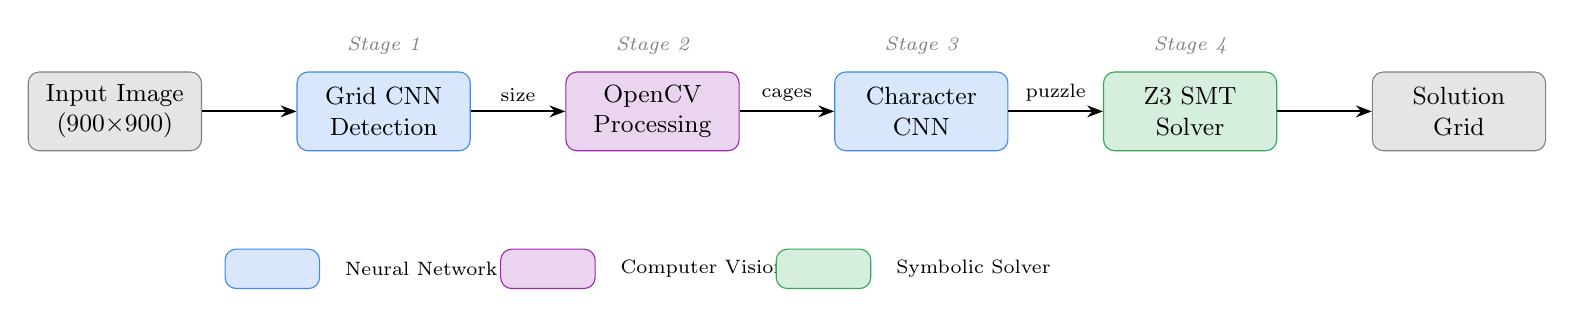
\begin{tikzpicture}[
    node distance=0.8cm and 1.2cm,
    box/.style={rectangle, draw, rounded corners, minimum width=2.2cm, minimum height=1cm, align=center, font=\small},
    neural/.style={box, fill=neuralblue!20, draw=neuralblue},
    cv/.style={box, fill=cvpurple!20, draw=cvpurple},
    symbolic/.style={box, fill=symbolicgreen!20, draw=symbolicgreen},
    io/.style={box, fill=gray!20, draw=gray},
    arrow/.style={-{Stealth[length=2mm]}, thick},
    label/.style={font=\scriptsize\itshape, text=gray}
]

% Input
\node[io] (input) {Input Image\\(900$\times$900)};

% Stage 1
\node[neural, right=of input] (grid) {Grid CNN\\Detection};
\node[label, above=0.1cm of grid] {Stage 1};

% Stage 2
\node[cv, right=of grid] (opencv) {OpenCV\\Processing};
\node[label, above=0.1cm of opencv] {Stage 2};

% Stage 3
\node[neural, right=of opencv] (char) {Character\\CNN};
\node[label, above=0.1cm of char] {Stage 3};

% Stage 4
\node[symbolic, right=of char] (z3) {Z3 SMT\\Solver};
\node[label, above=0.1cm of z3] {Stage 4};

% Output
\node[io, right=of z3] (output) {Solution\\Grid};

% Arrows with labels
\draw[arrow] (input) -- (grid);
\draw[arrow] (grid) -- node[above, font=\scriptsize] {size} (opencv);
\draw[arrow] (opencv) -- node[above, font=\scriptsize] {cages} (char);
\draw[arrow] (char) -- node[above, font=\scriptsize] {puzzle} (z3);
\draw[arrow] (z3) -- (output);

% Legend
\begin{scope}[shift={(0,-2)}]
    \node[neural, minimum width=1.2cm, minimum height=0.5cm] at (2,0) {};
    \node[right, font=\scriptsize] at (2.8,0) {Neural Network};

    \node[cv, minimum width=1.2cm, minimum height=0.5cm] at (5.5,0) {};
    \node[right, font=\scriptsize] at (6.3,0) {Computer Vision};

    \node[symbolic, minimum width=1.2cm, minimum height=0.5cm] at (9,0) {};
    \node[right, font=\scriptsize] at (9.8,0) {Symbolic Solver};
\end{scope}

\end{tikzpicture}
\caption{Neuro-symbolic pipeline architecture. Neural components (blue) handle perception while the symbolic solver (green) performs constraint satisfaction.}
\label{fig:architecture}
\end{figure}

\subsubsection{Stage 1: Grid Size Detection}

A convolutional neural network classifies the input image to determine puzzle dimensions (3$\times$3 through 9$\times$9). This information is essential for subsequent processing stages.

\subsubsection{Stage 2: Structure Extraction (OpenCV)}

Computer vision algorithms detect cage boundaries and cell locations:
\begin{itemize}[noitemsep]
    \item \textbf{Edge Enhancement}: \texttt{pyrMeanShiftFiltering} with spatial radius 5 and color radius 40
    \item \textbf{Edge Detection}: Canny algorithm with thresholds (50, 200)
    \item \textbf{Line Detection}: Probabilistic Hough Transform (\texttt{HoughLinesP}) with threshold 75
    \item \textbf{Cage Construction}: BFS-based region growing to identify contiguous cell groups
\end{itemize}

\subsubsection{Stage 3: Character Recognition}

A second CNN recognizes digits (0-9) and operators (+, $-$, $\times$, $\div$) from extracted cell regions. Characters are normalized to 28$\times$28 grayscale images before classification.

\subsubsection{Stage 4: Constraint Solving}

The Z3 SMT solver receives the extracted puzzle structure and computes valid solutions using formal constraints. Optimization techniques including singleton pre-filling and domain tightening accelerate solving.

\subsection{Neural Network Architectures}
\label{sec:networks}

Both CNNs follow a similar architecture with modifications for their respective input sizes and output classes.

\begin{table}[H]
\centering
\caption{Neural Network Architectures}
\label{tab:architectures}
\begin{tabular}{@{}lcc@{}}
\toprule
\textbf{Component} & \textbf{Grid CNN} & \textbf{Character CNN} \\
\midrule
Input Size & 128$\times$128$\times$1 & 28$\times$28$\times$1 \\
Conv Layer 1 & 32 filters, 3$\times$3 & 32 filters, 3$\times$3 \\
Conv Layer 2 & 64 filters, 3$\times$3 & 64 filters, 3$\times$3 \\
Pooling & MaxPool 2$\times$2 & MaxPool 2$\times$2 (per conv) \\
Dropout & 0.25 & 0.25 \\
FC Layer 1 & 262,144 $\rightarrow$ 128 & 3,136 $\rightarrow$ 128 \\
FC Layer 2 & 128 $\rightarrow$ 5-6 & 128 $\rightarrow$ 14 \\
Activation & ReLU + Softmax & ReLU + Softmax \\
\midrule
Output Classes & Sizes 3-7 (or 3-9) & 0-9, +, $-$, $\times$, $\div$ \\
\bottomrule
\end{tabular}
\end{table}

\subsubsection{Training Data}

\begin{itemize}[noitemsep]
    \item \textbf{Grid CNN}: Trained on generated puzzle images with known sizes
    \item \textbf{Character CNN (Printed)}: TMNIST dataset (NotoSans font) with custom operator symbols
    \item \textbf{Character CNN (Handwritten)}: MNIST for digits 0-9, EMNIST-Letters for A-G (HexaSudoku)
\end{itemize}

\subsection{Z3 Constraint Formulation}
\label{sec:constraints}

\subsubsection{KenKen Constraints}

For an $n \times n$ KenKen puzzle with cells $X_{i,j}$ where $1 \leq i,j \leq n$:

\begin{align}
\text{Cell Range:} \quad & 1 \leq X_{i,j} \leq n & \forall i,j \label{eq:range} \\
\text{Row Distinct:} \quad & \text{Distinct}(X_{i,1}, X_{i,2}, \ldots, X_{i,n}) & \forall i \label{eq:row} \\
\text{Column Distinct:} \quad & \text{Distinct}(X_{1,j}, X_{2,j}, \ldots, X_{n,j}) & \forall j \label{eq:col}
\end{align}

For each cage $C$ with cells $\{c_1, c_2, \ldots, c_k\}$, target $t$, and operator $\oplus$:

\begin{align}
\text{Addition:} \quad & \sum_{c \in C} X_c = t \\
\text{Multiplication:} \quad & \prod_{c \in C} X_c = t \\
\text{Subtraction:} \quad & |X_{c_1} - X_{c_2}| = t & (k=2) \\
\text{Division:} \quad & X_{c_1} = t \cdot X_{c_2} \lor X_{c_2} = t \cdot X_{c_1} & (k=2)
\end{align}

\subsubsection{Sudoku Constraints}

Standard Sudoku adds box constraints to the Latin square rules:

\begin{equation}
\text{Box Distinct:} \quad \text{Distinct}(\text{cells in box } B) \quad \forall B \in \text{Boxes}
\end{equation}

where boxes are 2$\times$2 for 4$\times$4 puzzles, 3$\times$3 for 9$\times$9, and 4$\times$4 for 16$\times$16 (HexaSudoku).

\subsubsection{Solver Optimizations}

We implement several optimizations to accelerate Z3 solving:

\begin{enumerate}[noitemsep]
    \item \textbf{Singleton Pre-filling}: Extract known values from single-cell cages, reducing variable count by 10-20\%
    \item \textbf{Integer-Only Division}: Avoid Z3's Real arithmetic by reformulating division as integer multiplication
    \item \textbf{Domain Tightening}: For addition cages with sum $t$ and $k$ cells, constrain each cell $\leq t - (k-1)$
    \item \textbf{Divisor Constraints}: For multiplication cages, each cell must divide the target
    \item \textbf{Solver Tactics}: Apply Z3's \texttt{simplify}, \texttt{propagate-values}, \texttt{solve-eqs}, then \texttt{smt}
\end{enumerate}

% ============================================
% SECTION 4: EXPERIMENTS
% ============================================
\section{Experiments}
\label{sec:experiments}

\subsection{Puzzle Datasets}
\label{sec:datasets}

\begin{table}[H]
\centering
\caption{Puzzle Dataset Summary}
\label{tab:datasets}
\begin{tabular}{@{}lccc@{}}
\toprule
\textbf{Puzzle Type} & \textbf{Sizes} & \textbf{Count per Size} & \textbf{Total} \\
\midrule
KenKen (Printed) & 3$\times$3 to 9$\times$9 & 100 each & 600 \\
Sudoku (Printed) & 4$\times$4, 9$\times$9 & 100 each & 200 \\
HexaSudoku (Printed) & 16$\times$16 & 100 & 100 \\
\midrule
Sudoku (Handwritten) & 4$\times$4, 9$\times$9 & 100 each & 200 \\
HexaSudoku (Handwritten) & 16$\times$16 & 100 & 100 \\
\bottomrule
\end{tabular}
\end{table}

All puzzles are generated using Z3 to guarantee unique solutions. Board images are rendered at 900$\times$900 pixels with consistent formatting.

\subsection{Printed Puzzle Evaluation}
\label{sec:printed}

\subsubsection{KenKen Results}

\begin{table}[H]
\centering
\caption{KenKen Neuro-Symbolic Solver Performance}
\label{tab:kenken-results}
\begin{tabular}{@{}ccccc@{}}
\toprule
\textbf{Size} & \textbf{Accuracy} & \textbf{Avg Time (ms)} & \textbf{Min (ms)} & \textbf{Max (ms)} \\
\midrule
3$\times$3 & 100\% & 143.6 & 89 & 312 \\
4$\times$4 & 100\% & 167.6 & 102 & 421 \\
5$\times$5 & 100\% & 204.4 & 134 & 589 \\
6$\times$6 & 100\% & 293.8 & 178 & 842 \\
7$\times$7 & 95\% & 511.0 & 245 & 2,890 \\
9$\times$9 & 62\% & $\sim$2,000 & 280 & 60,000 \\
\bottomrule
\end{tabular}
\end{table}

The 7$\times$7 accuracy drop (95\%) is attributed to occasional CNN misrecognition of cage boundaries. The 9$\times$9 accuracy (62\%) reflects increased character recognition errors and cage complexity.

\subsubsection{Sudoku Results}

\begin{table}[H]
\centering
\caption{Sudoku Neuro-Symbolic Solver Performance}
\label{tab:sudoku-results}
\begin{tabular}{@{}cccccc@{}}
\toprule
\textbf{Size} & \textbf{Accuracy} & \textbf{Avg Time (ms)} & \textbf{Min (ms)} & \textbf{Max (ms)} & \textbf{Std Dev} \\
\midrule
4$\times$4 & 100\% & 26.99 & 20.57 & 134.04 & 14.27 \\
9$\times$9 & 100\% & 275.06 & 130.70 & 605.63 & 99.40 \\
\bottomrule
\end{tabular}
\end{table}

Sudoku achieves 100\% accuracy on both sizes, benefiting from simpler structure (fixed grid, no cage detection) and purely distinctness constraints.

\subsection{Handwritten Digit Recognition}
\label{sec:handwritten}

We evaluate handwritten puzzle solving using multiple train/test splits of MNIST and EMNIST data.

\subsubsection{Dataset Configurations}

\begin{table}[H]
\centering
\caption{Handwritten Dataset Splits}
\label{tab:splits}
\begin{tabular}{@{}lccl@{}}
\toprule
\textbf{Split} & \textbf{Train/Class} & \textbf{Test/Class} & \textbf{Description} \\
\midrule
83-17 & 5,000 & 1,000 & Original experiments \\
90-10 & 5,400 & 600 & More training data \\
95-5 & 5,700 & 300 & Maximum training data \\
100-0 & $\sim$7,000 & 0 & Upper bound (board uses train) \\
\bottomrule
\end{tabular}
\end{table}

\subsubsection{Recognition and Solve Rates}

\begin{table}[H]
\centering
\caption{Handwritten Puzzle Results (Without Error Correction)}
\label{tab:handwritten-base}
\begin{tabular}{@{}lcccc@{}}
\toprule
\textbf{Puzzle Type} & \textbf{Split} & \textbf{Char Accuracy} & \textbf{Solve Rate} \\
\midrule
Sudoku 4$\times$4 & 83-17 & 99.50\% & 92\% \\
Sudoku 4$\times$4 & 90-10 & 99.31\% & 92\% \\
Sudoku 9$\times$9 & 83-17 & 99.67\% & 79\% \\
Sudoku 9$\times$9 & 90-10 & 99.64\% & 75\% \\
HexaSudoku 16$\times$16 & 83-17 & 98.89\% & 6\% \\
HexaSudoku 16$\times$16 & 90-10 & 99.06\% & 10\% \\
\bottomrule
\end{tabular}
\end{table}

\textbf{Key Observation}: Even with 99\%+ character recognition accuracy, solve rates drop significantly for larger puzzles. A single misrecognized digit can make the entire puzzle unsolvable due to conflicting constraints.

\subsection{Error Detection and Correction}
\label{sec:error-correction}

We develop three strategies to recover from CNN misclassifications.

\subsubsection{Method 1: Confidence-Based Correction}

Uses CNN softmax probabilities to identify likely errors:
\begin{enumerate}[noitemsep]
    \item Sort recognized clues by confidence (lowest first)
    \item Substitute each suspect with its second-best prediction
    \item Try single-error, then two-error corrections exhaustively
\end{enumerate}

\subsubsection{Method 2: Constraint-Based Correction (Unsat Core)}

Uses Z3's \texttt{unsat\_core()} to identify logically conflicting clues:
\begin{enumerate}[noitemsep]
    \item Attempt solve; if UNSAT, extract minimal conflicting constraint set
    \item For each suspect clue, temporarily remove and re-solve
    \item Rank suspects by conflict frequency across probes
    \item Substitute alternatives from CNN's second-best prediction
\end{enumerate}

\subsubsection{Method 3: Top-K Prediction}

Extends constraint-based approach by trying 2nd, 3rd, and 4th best CNN predictions:
\begin{enumerate}[noitemsep]
    \item When second-best prediction fails, try additional alternatives
    \item Supports up to 5-error correction with targeted search
\end{enumerate}

\begin{figure}[H]
\centering
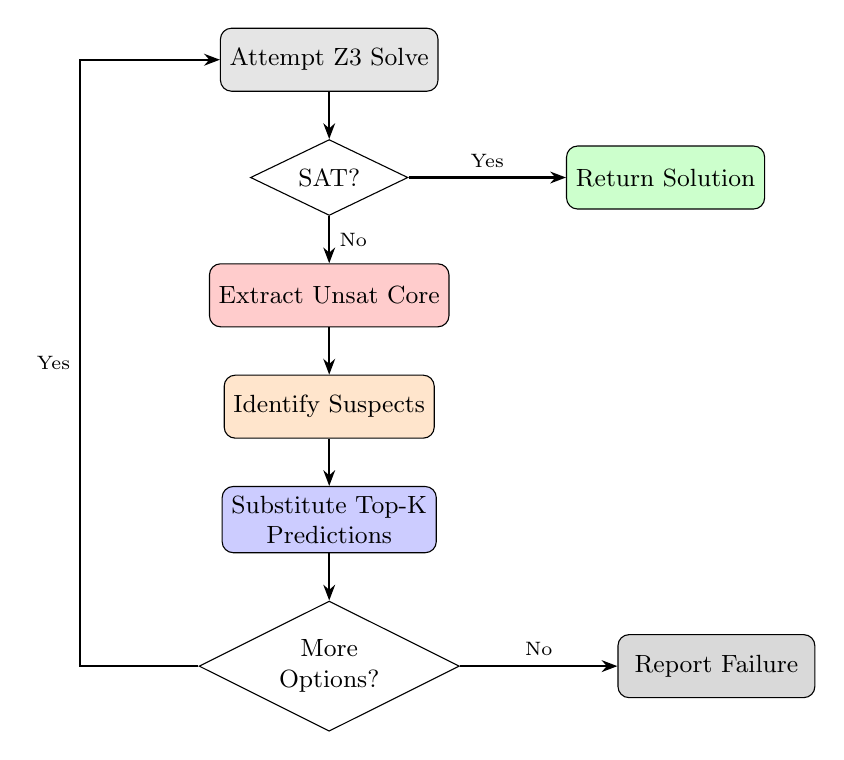
\begin{tikzpicture}[
    node distance=0.6cm and 1cm,
    box/.style={rectangle, draw, rounded corners, minimum width=2.5cm, minimum height=0.8cm, align=center, font=\small},
    decision/.style={diamond, draw, aspect=2, minimum width=2cm, align=center, font=\small},
    arrow/.style={-{Stealth[length=2mm]}, thick}
]

% Nodes
\node[box, fill=gray!20] (start) {Attempt Z3 Solve};
\node[decision, below=of start] (sat) {SAT?};
\node[box, fill=green!20, right=2cm of sat] (done) {Return Solution};
\node[box, fill=red!20, below=of sat] (unsat) {Extract Unsat Core};
\node[box, fill=orange!20, below=of unsat] (suspects) {Identify Suspects};
\node[box, fill=blue!20, below=of suspects] (substitute) {Substitute Top-K\\Predictions};
\node[decision, below=of substitute] (retry) {More\\Options?};
\node[box, fill=gray!30, right=2cm of retry] (fail) {Report Failure};

% Arrows
\draw[arrow] (start) -- (sat);
\draw[arrow] (sat) -- node[above, font=\scriptsize] {Yes} (done);
\draw[arrow] (sat) -- node[right, font=\scriptsize] {No} (unsat);
\draw[arrow] (unsat) -- (suspects);
\draw[arrow] (suspects) -- (substitute);
\draw[arrow] (substitute) -- (retry);
\draw[arrow] (retry) -- node[above, font=\scriptsize] {No} (fail);
\draw[arrow] (retry.west) -- ++(-1.5,0) |- node[left, font=\scriptsize, pos=0.25] {Yes} (start.west);

\end{tikzpicture}
\caption{Error correction workflow using unsat core analysis and Top-K substitution.}
\label{fig:error-correction}
\end{figure}

\subsubsection{Error Correction Comparison}

\begin{table}[H]
\centering
\caption{Error Correction Method Comparison (90-10 Split)}
\label{tab:error-correction}
\begin{tabular}{@{}lccc@{}}
\toprule
\textbf{Aspect} & \textbf{Confidence} & \textbf{Unsat Core} & \textbf{+ Top-K} \\
\midrule
Principle & Statistical & Logical & Logical + Multi-pred \\
Max Errors Corrected & 2 & 5 & 5 \\
\midrule
Sudoku 4$\times$4 & 99\% & 99\% & 99\% \\
Sudoku 9$\times$9 & \textbf{99\%} & 85\% & 84\% \\
HexaSudoku 16$\times$16 & 37\% & 36\% & \textbf{40\%} \\
\midrule
Avg Solver Calls & 50-500 & \textbf{2-20} & 2-800 \\
\bottomrule
\end{tabular}
\end{table}

\textbf{Key Findings}:
\begin{itemize}[noitemsep]
    \item Confidence-based excels on 9$\times$9 Sudoku (catches ``invisible'' errors)
    \item Unsat core is 10-25$\times$ faster but misses non-conflicting errors
    \item Top-K improves HexaSudoku by 4\% when second-best is also wrong
\end{itemize}

\subsection{Digits-Only Experiment}
\label{sec:digits-only}

An alternative approach renders HexaSudoku values 10-16 as two-digit numbers (e.g., ``16'' instead of letter ``G''), using only MNIST-trained digit recognition.

\subsubsection{Domain Constraint Enforcement}

\begin{itemize}[noitemsep]
    \item \textbf{Tens Digit}: Forced to 1 (all values 10-16 start with ``1'')
    \item \textbf{Ones Digit}: Constrained to 0-6 (values 17-19 don't exist)
    \item \textbf{Alternative Filtering}: Error correction only considers valid values $\{10, 11, \ldots, 16\}$
\end{itemize}

\begin{table}[H]
\centering
\caption{Digits-Only vs Letters Comparison (90-10 Split)}
\label{tab:digits-only}
\begin{tabular}{@{}lccc@{}}
\toprule
\textbf{Metric} & \textbf{Letters (A-G)} & \textbf{Digits Only} & \textbf{+ Domain} \\
\midrule
Top-K Solve Rate & 40\% & 34\% & \textbf{58\%} \\
Constraint-Based Solve & 36\% & 22\% & \textbf{49\%} \\
Cell Error Rate (10-16) & $\sim$1\% & 4.7\% & $\sim$1.5\% \\
\bottomrule
\end{tabular}
\end{table}

Domain constraints improve solve rate from 34\% to 58\% (+71\% relative improvement) by eliminating impossible values during recognition.

\subsection{Upper Bound Analysis (100-0 Split)}
\label{sec:upper-bound}

Using all available MNIST/EMNIST data for training and generating board images from training samples (i.e., CNN has ``seen'' all characters):

\begin{table}[H]
\centering
\caption{Upper Bound Results (100-0 Split)}
\label{tab:upper-bound}
\begin{tabular}{@{}lcc@{}}
\toprule
\textbf{Puzzle Type} & \textbf{Solve Rate} & \textbf{Avg Errors/Puzzle} \\
\midrule
HexaSudoku 16$\times$16 & 68\% & 1.45 \\
\bottomrule
\end{tabular}
\end{table}

\textbf{Key Insight}: Even with ``perfect familiarity'' (training data), solve rate is only 68\%, not 100\%. This is because data augmentation during training (rotation, scaling) creates variations that don't exactly match board images.

% ============================================
% SECTION 5: LLM BENCHMARK COMPARISON
% ============================================
\section{LLM Benchmark Comparison}
\label{sec:llm}

\subsection{Methodology}
\label{sec:llm-method}

We evaluate four leading vision-language models on KenKen puzzle solving:

\begin{itemize}[noitemsep]
    \item \textbf{Claude Sonnet 4} (claude-sonnet-4-20250514) via Anthropic API
    \item \textbf{GPT-4o Mini} (gpt-4o-mini) via OpenAI API
    \item \textbf{Gemini 2.5 Pro} via Google AI API
    \item \textbf{Qwen 2.5 VL} via local Hugging Face Transformers
\end{itemize}

\subsubsection{Prompt Design}

All models receive identical prompts describing KenKen rules:

\begin{quote}
\small\ttfamily
``You will be provided an empty KenKen puzzle board... every row and column must contain the numbers 1 through n. The thick border lines represent cages with a target number and arithmetic operator (+-/*). For a given cage, all numbers must arrive at the target through the operator... Format your response as a 2 dimensional list representing the solution for the puzzle.''
\end{quote}

\subsubsection{Validation}

LLM outputs are validated using Z3 against the same constraints as our neuro-symbolic solver, ensuring fair comparison.

\subsection{Results}
\label{sec:llm-results}

\begin{table}[H]
\centering
\caption{LLM vs Neuro-Symbolic Accuracy on KenKen (30 puzzles per size)}
\label{tab:llm-comparison}
\begin{tabular}{@{}lcccccc@{}}
\toprule
\textbf{Solver} & \textbf{3$\times$3} & \textbf{4$\times$4} & \textbf{5$\times$5} & \textbf{6$\times$6} & \textbf{7$\times$7} & \textbf{Avg Time} \\
\midrule
\textbf{NeuroSymbolic} & \textbf{100\%} & \textbf{100\%} & \textbf{100\%} & \textbf{100\%} & \textbf{95\%} & $\sim$0.3s \\
\midrule
Gemini 2.5 Pro & 74\% & 30\% & 0\% & 0\% & 0\% & $\sim$238s \\
Claude Sonnet 4 & 39\% & 7\% & 0\% & 0\% & 0\% & $\sim$24s \\
Qwen 2.5 VL & 10\% & 0\% & 0\% & 0\% & 0\% & $\sim$46s \\
GPT-4o Mini & 8\% & 0\% & 0\% & 0\% & 0\% & $\sim$4s \\
\bottomrule
\end{tabular}
\end{table}

\begin{figure}[H]
\centering
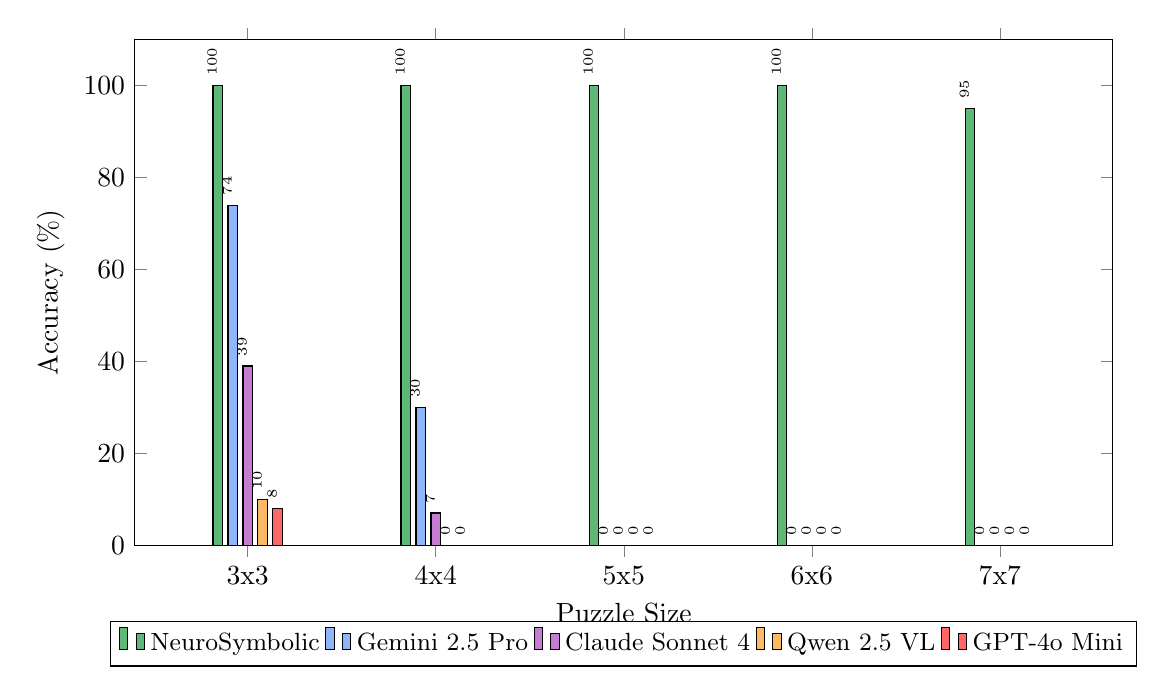
\begin{tikzpicture}
\begin{axis}[
    ybar,
    bar width=0.12cm,
    width=14cm,
    height=8cm,
    ylabel={Accuracy (\%)},
    xlabel={Puzzle Size},
    symbolic x coords={3x3, 4x4, 5x5, 6x6, 7x7},
    xtick=data,
    ymin=0, ymax=110,
    legend style={at={(0.5,-0.15)}, anchor=north, legend columns=5, font=\small},
    nodes near coords,
    nodes near coords style={font=\tiny, rotate=90, anchor=west},
    every node near coord/.append style={yshift=2pt},
    enlarge x limits=0.15,
]
\addplot[fill=symbolicgreen!80] coordinates {(3x3,100) (4x4,100) (5x5,100) (6x6,100) (7x7,95)};
\addplot[fill=neuralblue!60] coordinates {(3x3,74) (4x4,30) (5x5,0) (6x6,0) (7x7,0)};
\addplot[fill=cvpurple!60] coordinates {(3x3,39) (4x4,7) (5x5,0) (6x6,0) (7x7,0)};
\addplot[fill=resultsorange!60] coordinates {(3x3,10) (4x4,0) (5x5,0) (6x6,0) (7x7,0)};
\addplot[fill=red!60] coordinates {(3x3,8) (4x4,0) (5x5,0) (6x6,0) (7x7,0)};
\legend{NeuroSymbolic, Gemini 2.5 Pro, Claude Sonnet 4, Qwen 2.5 VL, GPT-4o Mini}
\end{axis}
\end{tikzpicture}
\caption{Accuracy comparison across puzzle sizes. All LLMs achieve 0\% accuracy on puzzles 5$\times$5 and larger.}
\label{fig:llm-bar}
\end{figure}

\subsection{Response Time Analysis}

\begin{table}[H]
\centering
\caption{Average Response Time per Puzzle (seconds)}
\label{tab:response-times}
\begin{tabular}{@{}lccccc@{}}
\toprule
\textbf{Solver} & \textbf{3$\times$3} & \textbf{4$\times$4} & \textbf{5$\times$5} & \textbf{6$\times$6} & \textbf{7$\times$7} \\
\midrule
NeuroSymbolic & 0.14 & 0.17 & 0.21 & 0.29 & 0.51 \\
GPT-4o Mini & 3.8 & 2.6 & 3.4 & 3.4 & 4.5 \\
Claude Sonnet 4 & 26.5 & 27.0 & 24.5 & 22.2 & 21.7 \\
Qwen 2.5 VL & 26.6 & 35.2 & 55.9 & 55.0 & 56.9 \\
Gemini 2.5 Pro & 145.4 & 240.9 & 249.9 & 276.4 & 279.1 \\
\bottomrule
\end{tabular}
\end{table}

The neuro-symbolic solver is \textbf{50-600$\times$ faster} than LLMs while achieving vastly higher accuracy.

\subsection{Failure Mode Analysis}

LLM failures exhibit consistent patterns:
\begin{itemize}[noitemsep]
    \item \textbf{Constraint Violations}: Solutions frequently violate Latin square or cage constraints
    \item \textbf{Impossible Values}: Models sometimes propose values outside the valid range (e.g., 8 in a 4$\times$4 puzzle)
    \item \textbf{Incomplete Reasoning}: Chain-of-thought shows logical gaps and inconsistent constraint application
    \item \textbf{No Backtracking}: Models cannot systematically explore the solution space when initial guesses fail
\end{itemize}

% ============================================
% SECTION 6: ANALYSIS AND DISCUSSION
% ============================================
\section{Analysis and Discussion}
\label{sec:analysis}

\subsection{Why LLMs Fail at Constraint Satisfaction}

Large language models are fundamentally probabilistic sequence predictors trained to maximize next-token likelihood. This architecture creates several limitations for constraint satisfaction:

\begin{enumerate}[noitemsep]
    \item \textbf{No Systematic Search}: LLMs generate outputs autoregressively without backtracking capability
    \item \textbf{Soft Constraints}: Training on natural language teaches soft preferences, not hard logical requirements
    \item \textbf{Exponential State Space}: A 5$\times$5 KenKen has $5^{25} \approx 3 \times 10^{17}$ possible configurations
    \item \textbf{Global Constraint Propagation}: Changing one cell affects constraints across the entire grid
\end{enumerate}

\subsection{Division of Labor in Neuro-Symbolic Systems}

Our results validate the neuro-symbolic paradigm's division of labor:

\begin{table}[H]
\centering
\caption{Task Decomposition: Neural vs Symbolic}
\label{tab:division}
\begin{tabular}{@{}lcc@{}}
\toprule
\textbf{Task} & \textbf{Best Approach} & \textbf{Reasoning} \\
\midrule
Grid size detection & Neural & Pattern recognition \\
Character recognition & Neural & Perceptual invariance \\
Cage boundary detection & CV + Neural & Edge detection + classification \\
Constraint propagation & Symbolic & Formal deduction \\
Solution search & Symbolic & Systematic backtracking \\
Error correction & Hybrid & CNN confidence + Z3 core \\
\bottomrule
\end{tabular}
\end{table}

\subsection{Handwritten Recognition Error Analysis}

The gap between character recognition accuracy (99\%) and puzzle solve rate (75-92\% for 9$\times$9 Sudoku) reveals a critical insight: \textbf{constraint satisfaction is brittle to input errors}. In a 9$\times$9 Sudoku with $\sim$25 clues:
\begin{itemize}[noitemsep]
    \item 99\% accuracy $\rightarrow$ expected 0.25 errors per puzzle
    \item A single error can make the puzzle unsolvable (conflicting constraints)
    \item Some errors are ``invisible'' (enable a different valid solution)
\end{itemize}

This brittleness motivates our error correction strategies, which recover 7-24\% of initially failed puzzles.

\subsection{Scalability Observations}

\begin{itemize}[noitemsep]
    \item \textbf{Z3 Scaling}: Solve time increases sublinearly with cell count (10.2$\times$ time for 5.1$\times$ cells in Sudoku)
    \item \textbf{LLM Scaling}: Response time roughly constant regardless of puzzle size (model capacity limitation)
    \item \textbf{Error Correction}: Unsat core approach scales better (2-20 calls vs 50-500) for larger puzzles
\end{itemize}

% ============================================
% SECTION 7: CONCLUSION
% ============================================
\section{Conclusion}
\label{sec:conclusion}

\subsection{Key Findings}

\begin{enumerate}
    \item \textbf{Neuro-Symbolic Superiority}: Our hybrid approach achieves 93-100\% accuracy on KenKen puzzles where the best LLM (Gemini 2.5 Pro) achieves 0-74\%.

    \item \textbf{Complete LLM Failure}: All tested LLMs fail completely (0\%) on puzzles 5$\times$5 and larger, demonstrating a fundamental limitation in constraint satisfaction.

    \item \textbf{Efficiency}: The neuro-symbolic solver is 50-600$\times$ faster than LLM solutions.

    \item \textbf{Error Correction}: Constraint-based error detection using Z3's unsat core achieves 10-25$\times$ faster correction than exhaustive approaches.

    \item \textbf{Domain Knowledge}: Integrating domain constraints into recognition improves solve rates by 24\% absolute (34\% $\rightarrow$ 58\%).
\end{enumerate}

\subsection{Implications for Neuro-Symbolic AI}

Our results demonstrate that:
\begin{itemize}[noitemsep]
    \item Hybrid architectures can outperform end-to-end neural approaches for structured reasoning
    \item The ``neural perception, symbolic reasoning'' paradigm is effective for constraint satisfaction
    \item Error correction benefits from combining statistical (CNN confidence) and logical (unsat core) signals
\end{itemize}

\subsection{Limitations}

\begin{itemize}[noitemsep]
    \item CNNs require retraining for new visual styles (fonts, handwriting)
    \item OpenCV pipeline assumes clean, well-formatted puzzle images
    \item Error correction cannot recover from multiple correlated errors affecting the same constraint
\end{itemize}

\subsection{Future Work}

\begin{itemize}[noitemsep]
    \item Extension to additional puzzle types (Kakuro, Killer Sudoku)
    \item End-to-end differentiable constraint layers for joint training
    \item Active learning for error correction (learning which substitutions succeed)
    \item Real-time mobile application for puzzle solving
\end{itemize}

% ============================================
% REFERENCES
% ============================================
\section*{References}

\begin{thebibliography}{9}

\bibitem{garcez2019neural}
Garcez, A. d., \& Lamb, L. C. (2020). Neurosymbolic AI: The 3rd wave. \textit{arXiv preprint arXiv:2012.05876}.

\bibitem{demoura2008z3}
De Moura, L., \& Bj{\o}rner, N. (2008). Z3: An efficient SMT solver. In \textit{International Conference on Tools and Algorithms for the Construction and Analysis of Systems} (pp. 337-340). Springer.

\bibitem{wei2022chain}
Wei, J., Wang, X., Schuurmans, D., et al. (2022). Chain-of-thought prompting elicits reasoning in large language models. \textit{Advances in Neural Information Processing Systems, 35}, 24824-24837.

\bibitem{babu2010sudoku}
Babu, K., Vijayalakshmi, S., \& Nedunchezhian, R. (2010). Recognition of handwritten Sudoku puzzles. \textit{International Journal of Computer Applications}, 1(4), 41-48.

\bibitem{lecun1998mnist}
LeCun, Y., Bottou, L., Bengio, Y., \& Haffner, P. (1998). Gradient-based learning applied to document recognition. \textit{Proceedings of the IEEE}, 86(11), 2278-2324.

\bibitem{cohen2017emnist}
Cohen, G., Afshar, S., Tapson, J., \& Van Schaik, A. (2017). EMNIST: Extending MNIST to handwritten letters. \textit{2017 International Joint Conference on Neural Networks (IJCNN)}, 2921-2926.

\end{thebibliography}

% ============================================
% APPENDIX
% ============================================
\newpage
\appendix

\section{Detailed CNN Architectures}
\label{app:cnn}

\subsection{Grid Detection CNN (PyTorch)}

\begin{lstlisting}[language=Python, caption=Grid CNN Architecture]
class Grid_CNN(nn.Module):
    def __init__(self, output_dim):
        super(Grid_CNN, self).__init__()
        self.conv1 = nn.Conv2d(1, 32, kernel_size=3, padding=1)
        self.conv2 = nn.Conv2d(32, 64, kernel_size=3, padding=1)
        self.pool = nn.MaxPool2d(2, 2)
        self.dropout = nn.Dropout(0.25)
        self.fc1 = nn.Linear(262144, 128)
        self.fc2 = nn.Linear(128, output_dim)

    def forward(self, x):
        x = F.relu(self.conv1(x))
        x = F.relu(self.conv2(x))
        x = self.pool(x)
        x = self.pool(x)
        x = self.dropout(x)
        x = x.view(x.size(0), -1)
        x = F.relu(self.fc1(x))
        x = self.fc2(x)
        return x
\end{lstlisting}

\subsection{Character Recognition CNN (PyTorch)}

\begin{lstlisting}[language=Python, caption=Character CNN Architecture]
class CNN_v2(nn.Module):
    def __init__(self, output_dim):
        super(CNN_v2, self).__init__()
        self.conv1 = nn.Conv2d(1, 32, kernel_size=3, padding=1)
        self.conv2 = nn.Conv2d(32, 64, kernel_size=3, padding=1)
        self.pool = nn.MaxPool2d(2, 2)
        self.dropout = nn.Dropout(0.25)
        self.fc1 = nn.Linear(3136, 128)
        self.fc2 = nn.Linear(128, output_dim)

    def forward(self, x):
        x = self.pool(F.relu(self.conv1(x)))
        x = self.pool(F.relu(self.conv2(x)))
        x = self.dropout(x)
        x = x.view(x.size(0), -1)
        x = F.relu(self.fc1(x))
        x = self.fc2(x)
        return x
\end{lstlisting}

\section{Z3 Constraint Pseudocode}
\label{app:z3}

\begin{algorithm}[H]
\caption{KenKen Z3 Constraint Generation}
\label{alg:z3}
\begin{algorithmic}[1]
\Require Puzzle $P$ with size $n$, cages $C$
\Ensure Solution grid $X$ or UNSAT
\State $X \gets$ matrix of Z3 Int variables $X_{i,j}$ for $i,j \in [0, n)$
\State $constraints \gets \emptyset$
\For{$i \in [0, n)$, $j \in [0, n)$}
    \State $constraints$.add($1 \leq X_{i,j} \leq n$) \Comment{Cell range}
\EndFor
\For{$i \in [0, n)$}
    \State $constraints$.add(Distinct($X_{i,*}$)) \Comment{Row uniqueness}
\EndFor
\For{$j \in [0, n)$}
    \State $constraints$.add(Distinct($X_{*,j}$)) \Comment{Column uniqueness}
\EndFor
\For{cage $(cells, op, target) \in C$}
    \If{$op = $ ``add''}
        \State $constraints$.add($\sum_{(i,j) \in cells} X_{i,j} = target$)
    \ElsIf{$op = $ ``mul''}
        \State $constraints$.add($\prod_{(i,j) \in cells} X_{i,j} = target$)
    \ElsIf{$op = $ ``sub'' and $|cells| = 2$}
        \State $(a, b) \gets cells$
        \State $constraints$.add($X_a - X_b = target \lor X_b - X_a = target$)
    \ElsIf{$op = $ ``div'' and $|cells| = 2$}
        \State $(a, b) \gets cells$
        \State $constraints$.add($X_a = target \cdot X_b \lor X_b = target \cdot X_a$)
    \EndIf
\EndFor
\State $solver \gets$ Z3.Solver()
\State $solver$.add($constraints$)
\If{$solver$.check() $=$ SAT}
    \State \Return extract\_solution($solver$.model(), $X$)
\Else
    \State \Return UNSAT
\EndIf
\end{algorithmic}
\end{algorithm}

\section{Complete Experimental Results}
\label{app:results}

\begin{table}[H]
\centering
\caption{Full KenKen Benchmark Results (100 puzzles per size)}
\label{tab:full-kenken}
\begin{tabular}{@{}ccccccc@{}}
\toprule
\textbf{Size} & \textbf{Solved} & \textbf{Failed} & \textbf{Timeout} & \textbf{Accuracy} & \textbf{Avg (ms)} & \textbf{Max (ms)} \\
\midrule
3$\times$3 & 100 & 0 & 0 & 100.0\% & 143.6 & 312 \\
4$\times$4 & 100 & 0 & 0 & 100.0\% & 167.6 & 421 \\
5$\times$5 & 100 & 0 & 0 & 100.0\% & 204.4 & 589 \\
6$\times$6 & 100 & 0 & 0 & 100.0\% & 293.8 & 842 \\
7$\times$7 & 93 & 7 & 0 & 93.0\% & 511.0 & 2,890 \\
9$\times$9 & 62 & 37 & 1 & 62.0\% & 2,012 & 60,000 \\
\bottomrule
\end{tabular}
\end{table}

\begin{table}[H]
\centering
\caption{Handwritten Error Correction Complete Results}
\label{tab:full-error}
\begin{tabular}{@{}llccc@{}}
\toprule
\textbf{Puzzle} & \textbf{Split} & \textbf{Base} & \textbf{Confidence} & \textbf{Unsat+TopK} \\
\midrule
Sudoku 4$\times$4 & 83-17 & 92\% & 96\% & 96\% \\
Sudoku 4$\times$4 & 90-10 & 92\% & 99\% & 99\% \\
Sudoku 9$\times$9 & 83-17 & 79\% & 91\% & 89\% \\
Sudoku 9$\times$9 & 90-10 & 75\% & 99\% & 84\% \\
HexaSudoku 16$\times$16 & 83-17 & 6\% & 30\% & 32\% \\
HexaSudoku 16$\times$16 & 90-10 & 10\% & 37\% & 40\% \\
HexaSudoku 16$\times$16 & 95-5 & 8\% & 35\% & 42\% \\
HexaSudoku 16$\times$16 & 100-0 & 24\% & 62\% & 68\% \\
\bottomrule
\end{tabular}
\end{table}

\end{document}
